%%%%%%%%%%%%%%%%%%%%%%%%%%%%%%%%%%%%%%%%%
% Proposal
%
% Author:
% Son Nguyen
% snguyen7@stevens.edu
%%%%%%%%%%%%%%%%%%%%%%%%%%%%%%%%%%%%%%%%%
% !TEX root = proposal.tex

%----------------------------------------------------------------------------------------
%	PACKAGES AND OTHER DOCUMENT CONFIGURATIONS
%----------------------------------------------------------------------------------------

\documentclass[
	a4paper, % Paper size, use either a4paper or letterpaper
	10pt, % Default font size, can also use 11pt or 12pt, although this is not recommended
	unnumberedsections, % Comment to enable section numbering
	twoside, % Two side traditional mode where headers and footers change between odd and even pages, comment this option to make them fixed
]{LTJournalArticle}

\usepackage{float}

\addbibresource{sample.bib} % BibLaTeX bibliography file

\runninghead{Shortened Running Article Title} % A shortened article title to appear in the running head, leave this command empty for no running head

\footertext{\textit{Journal of Biological Sampling} (2024) 12:533-684} % Text to appear in the footer, leave this command empty for no footer text

\setcounter{page}{1} % The page number of the first page, set this to a higher number if the article is to be part of an issue or larger work

%----------------------------------------------------------------------------------------
%	TITLE SECTION
%----------------------------------------------------------------------------------------

\title{Summary: Performing Quantum Computation with Classical Optics} % Article title, use manual lines breaks (\\) to beautify the layout

% Authors are listed in a comma-separated list with superscript numbers indicating affiliations
% \thanks{} is used for any text that should be placed in a footnote on the first page, such as the corresponding author's email, journal acceptance dates, a copyright/license notice, keywords, etc
\author{%
	Xiaofeng Qian, Son H. Nguyen, Matthew Daddino, Ching Man Wong
}

% Affiliations are output in the \date{} command
\date{Physics Department, Stevens Institute of Technology, Hoboken, NJ 07030, USA}

% Full-width abstract
\renewcommand{\maketitlehookd}{%
	\begin{abstract}
		\noindent Quantum computers promise transformative capabilities for molecular simulation and optimization problems, yet practical implementations face significant technological barriers. This research demonstrates an alternative approach: implementing quantum algorithms using classical optical systems. We present a framework for performing quantum computation through optical components, specifically realizing the Variational Quantum Eigensolver (VQE) algorithm for molecular energy calculations. Our implementation encodes qubits using photonic polarization states and spatial modes, leveraging wave plates (quarter-wave and half-wave), beamsplitters, and dove prisms to construct quantum gates. We detail the theoretical decomposition of the UCCSD (Unitary Coupled Cluster Single and Double excitations) ansatz for the hydrogen molecule, deriving the necessary rotations and entangling operations. The optical realization employs Jones calculus to systematically map quantum gates onto polarization-dependent optical transformations, with Stokes vector measurements enabling quantum state readout. This hybrid classical-optical approach provides insights into quantum circuit implementation while leveraging the well-established optical laboratory infrastructure, demonstrating that quantum algorithms can be executed through photonic platforms as an alternative to superconducting or trapped-ion systems.
	\end{abstract}
}

%----------------------------------------------------------------------------------------

\begin{document}

\maketitle % Output the title section

%----------------------------------------------------------------------------------------
%	ARTICLE CONTENTS
%----------------------------------------------------------------------------------------

\section{Introduction}

Following O'Malley et al., we begin with the reduced two-qubit electronic Hamiltonian for molecular hydrogen:
\begin{equation}
\hat{H} = g_0 \mathbb{I} + g_1 Z_0 + g_2 Z_1 + g_3 Z_0 Z_1 + g_4 Y_0 Y_1 + g_5 X_0 X_1,
\label{eq:omalley_hamiltonian}
\end{equation}
where $X_i$, $Y_i$, and $Z_i$ are Pauli operators acting on qubit $i$, and the coefficients $g_k$ depend on molecular geometry (in particular, bond length). This compact form captures the essential electronic structure terms needed for ground-state estimation in a near-term quantum setting.

Estimating the minimum eigenvalue of Eq.~\ref{eq:omalley_hamiltonian} is the central task of the Variational Quantum Eigensolver (VQE): prepare a parameterized trial state, measure the expectation value $\langle \hat{H} \rangle$, and iteratively update parameters to approach the ground-state energy. In the standard digital model, this procedure is implemented with a reference state preparation, single-qubit rotations, and entangling gates that realize a UCC-inspired ansatz for H$_2$.

This thesis investigates how the same quantum-information workflow can be implemented using classical optics. We map qubit states to photonic degrees of freedom (polarization and spatial mode), and map unitary gate operations to physically realizable optical transformations built from wave plates, beam splitters, and mode-control elements. Jones-matrix and Stokes-parameter formalisms are used to connect the theoretical circuit operations to measurable optical quantities.

The goal is not to claim a universal quantum speedup with classical hardware, but to construct a physically transparent and experimentally accessible platform for studying quantum-circuit structure, variational optimization behavior, and measurement strategies motivated by quantum chemistry. By grounding the study in the O'Malley Hamiltonian and the H$_2$ VQE benchmark, this work provides a concrete bridge between quantum-algorithm design and optical laboratory realization.

%------------------------------------------------

\section{Preparation of the Quantum Circuit}
To implement the VQE algorithm for the Hamiltonian in Eq.~\ref{eq:omalley_hamiltonian}, we first need to prepare the quantum circuit that corresponds to the UCCSD ansatz for H$_2$. This involves decomposing the unitary operator into a sequence of single-qubit rotations and two-qubit entangling gates.

\begin{figure}[H]
\centering
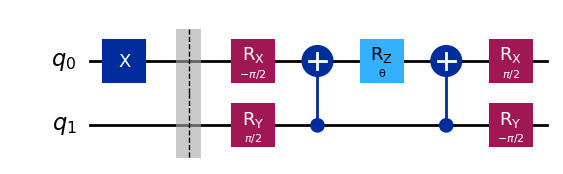
\includegraphics[width=0.85\linewidth]{Figures/Circ.png}
\caption{UCCSD ansatz circuit for the hydrogen molecule benchmark used in this work.}
\label{fig:uccsd-circuit}
\end{figure}
\section{Optical implementation of Quantum Gates}

%------------------------------------------------

%----------------------------------------------------------------------------------------
%	 REFERENCES
%----------------------------------------------------------------------------------------

\printbibliography % Output the bibliography

%----------------------------------------------------------------------------------------

\end{document}
